% Auto-generated by the analysis pipeline — do not edit
% y > 0: Overreacts  |  y < 0: Underreacts
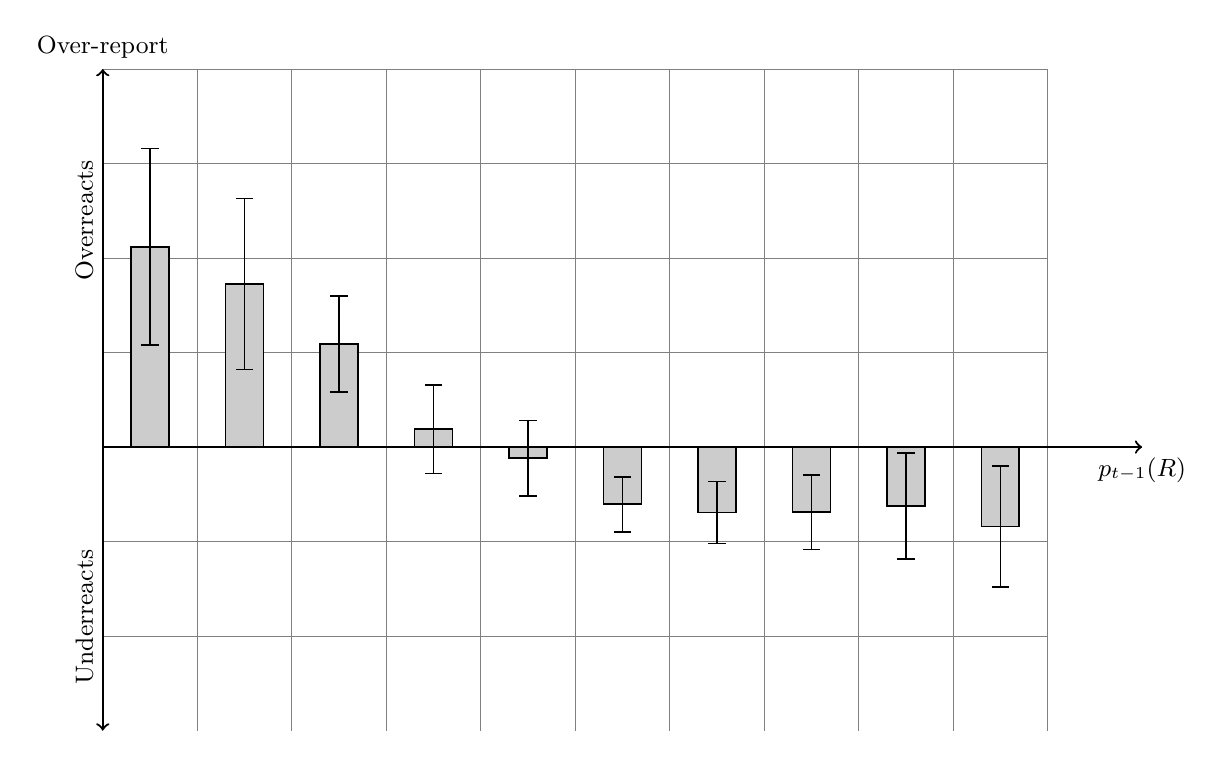
\begin{tikzpicture}[scale=12]
\draw[help lines,step=0.1] (0,-0.3) grid (1,0.4);
\filldraw[opaque,white!80!black] (0.03,0) rectangle (0.07,0.2119);
\draw[line width=0.6] (0.03,0) rectangle (0.07,0.2119);
\draw[line width=0.6,|-|] (0.05,0.1071) -- (0.05,0.3168);
\filldraw[opaque,white!80!black] (0.13,0) rectangle (0.17,0.1726);
\draw[line width=0.6] (0.13,0) rectangle (0.17,0.1726);
\draw[line width=0.6,|-|] (0.15,0.0811) -- (0.15,0.2640);
\filldraw[opaque,white!80!black] (0.23,0) rectangle (0.27,0.1089);
\draw[line width=0.6] (0.23,0) rectangle (0.27,0.1089);
\draw[line width=0.6,|-|] (0.25,0.0573) -- (0.25,0.1605);
\filldraw[opaque,white!80!black] (0.33,0) rectangle (0.37,0.0189);
\draw[line width=0.6] (0.33,0) rectangle (0.37,0.0189);
\draw[line width=0.6,|-|] (0.35,-0.0289) -- (0.35,0.0668);
\filldraw[opaque,white!80!black] (0.43,0) rectangle (0.47,-0.0117);
\draw[line width=0.6] (0.43,0) rectangle (0.47,-0.0117);
\draw[line width=0.6,|-|] (0.45,-0.0525) -- (0.45,0.0291);
\filldraw[opaque,white!80!black] (0.53,0) rectangle (0.57,-0.0606);
\draw[line width=0.6] (0.53,0) rectangle (0.57,-0.0606);
\draw[line width=0.6,|-|] (0.55,-0.0906) -- (0.55,-0.0306);
\filldraw[opaque,white!80!black] (0.63,0) rectangle (0.67,-0.0693);
\draw[line width=0.6] (0.63,0) rectangle (0.67,-0.0693);
\draw[line width=0.6,|-|] (0.65,-0.1030) -- (0.65,-0.0355);
\filldraw[opaque,white!80!black] (0.73,0) rectangle (0.77,-0.0690);
\draw[line width=0.6] (0.73,0) rectangle (0.77,-0.0690);
\draw[line width=0.6,|-|] (0.75,-0.1093) -- (0.75,-0.0287);
\filldraw[opaque,white!80!black] (0.83,0) rectangle (0.87,-0.0625);
\draw[line width=0.6] (0.83,0) rectangle (0.87,-0.0625);
\draw[line width=0.6,|-|] (0.85,-0.1197) -- (0.85,-0.0053);
\filldraw[opaque,white!80!black] (0.93,0) rectangle (0.97,-0.0840);
\draw[line width=0.6] (0.93,0) rectangle (0.97,-0.0840);
\draw[line width=0.6,|-|] (0.95,-0.1491) -- (0.95,-0.0189);
\draw[line width=0.8,->]  (0,0) -- (1.1,0) node[below] {\small{$p_{t-1}(R)$}};
\draw[line width=0.8,<->] (0,-0.3) -- (0,0.4) node[above] {\small{Over-report}};
\draw (0,0.24) node[above,rotate=90] {\small{Overreacts}};
\draw (0,-0.18) node[above,rotate=90] {\small{Underreacts}};
% ADD THEORY CURVE BELOW
\end{tikzpicture}
